% ---------------------------- Preamble starts here ----------------------------

\documentclass[aspectratio=169]{beamer} %Remove [aspectratio=169] to get non-wide 4:3 slide aspect ratio

% --- Set beamer theme
\usetheme{Metropolis}
\setbeamertemplate{footline}{}				% Remove automatic footer
\setbeamertemplate{navigation symbols}{}	% Comment this line to display navigation symbols

% Load i2i symbol
\addtobeamertemplate{frametitle}{}{%
\begin{textblock*}{\linewidth}(0cm,7.4cm) % Replace with (0cm, 8cm) if using non-wide slide aspect
	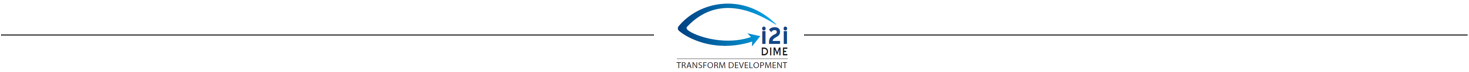
\includegraphics[width=\linewidth]{../img/Footer.png}
\end{textblock*}}

% --- Load packages
\usepackage{textpos}		% To align objects correctly
\usepackage{multicol}		% To right in multiple columns
\usepackage{color}			% To color text

% --- Add your information here
\title{Git Better - Understanding Git and GitHub}
\author{DIME Analytics}
\institute{DIME - The World Bank}
\date{\today}

\newcommand{\repoUserAndName}{kbjarkefur/lyrics}
\newcommand{\trainingRepoURL}[1]{\url{github.com/\repoUserAndName #1} }
\newcommand{\trainerEmail}{\url{kbjarkefur@worldbank.org} }

% ---------------------------- Preamble ends here ----------------------------

\begin{document}

\begin{frame}

\includegraphics[width=\textwidth]{../img/Header.png}
\vspace{-0.2cm}
\titlepage 	 % Opening slide, prints inform
\end{frame}


\begin{frame}
\frametitle{Git Better}
	The goal of this training:

	\begin{enumerate}
		\item Better understand the practices we recommend so that you can use them even better
		\item Not having to rely as much on DIME Analytics for 
		\begin{itemize}
			\item Understanding why something is happening
			\item Solve errors or warnings
			\item Setting up or customizing your own work flows
		\end{itemize} 
	\end{enumerate} 
\end{frame}

\begin{frame}
	\frametitle{Content}
	Four sections:
	
	\begin{enumerate}
		\item Git vs. GitHub
		\item Knowing Git better
		\item Knowing GitHub better
		\item Work flows
	\end{enumerate} 
\end{frame}

\section{Git vs. GitHub}

\begin{frame}
	\frametitle{Git features and GitHub features}
	\begin{columns}[c] 
	
		\column{.35\textwidth} % Left column and width
		It is important to start to think about which features comes from Git and which comes from your Git implementation, i.e. GitHub
		\vspace{.5cm}
		
		Git clients do not tend to add new features. Clients mostly differ in how features are displayed
		\column{.65\textwidth} % Right column and width
		\begin{figure}
			\centering
			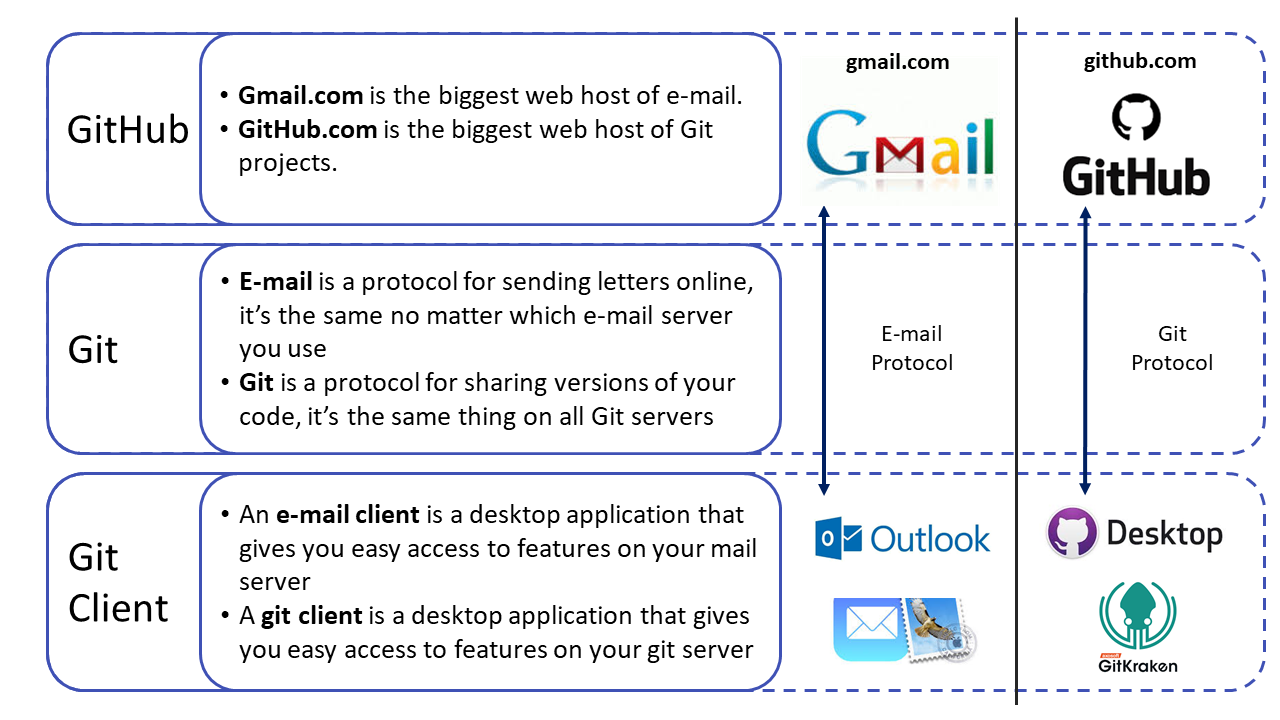
\includegraphics[width=1\linewidth]{../img/git_github_gitclient_gitclient}
			\label{fig:finaldoccartoon}
		\end{figure}
	\end{columns}
\end{frame}


\begin{frame}
	\frametitle{Git features and GitHub features}
		
	\begin{itemize}
		\item Features from Git itself changes very little. Updates that affects how we work with Git are very rare
		\item Features from GitHub changes a lot. While most changes are minor, they regularly change how some feature works. 
	\end{itemize}  
	
	When setting up your work flow it is ok if your project depends on features in Git, but if your project and its work flow depends too much on features in GitHub you run a risk to wake up one day.	Use the features in GitHub, they are great, just make sure to not depend on them.

\end{frame}

\begin{frame}
	\frametitle{Git features and GitHub features}
	
	\begin{itemize}
		\item DIME Analytics take this difference when we recommend work flows to teams
		\item And that is why this training are structured by first going over Git Features, and then GitHub Features
	\end{itemize}  
\end{frame}

\section{Know Git Better}

\section{Know GitHub Better}

\section{Work flow}

\end{document}
